\documentclass[border=4pt]{standalone}

% --- packages (mirror these in convolution.meta.json "requires") ---
\usepackage{tikz}
\usetikzlibrary{arrows.meta}

% --- palette (canonical source: reference/color-palettes/color-palettes.md; light variant) ---
\definecolor{otblue}{HTML}{0072B2}
\definecolor{otorange}{HTML}{E69F00}
\definecolor{otteal}{HTML}{009E73}
\definecolor{otpurple}{HTML}{CC79A7}
\definecolor{otgray}{HTML}{5A5A5A}

\begin{document}
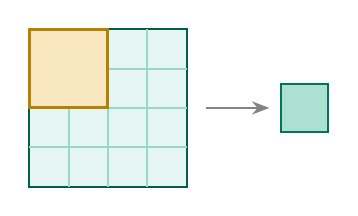
\begin{tikzpicture}[line width=0.7pt, >={Stealth[length=2.2mm]}]
  % input feature map (4x4 grid)
  \draw[draw=otteal!60!black, fill=otteal!10] (0,0) rectangle (2,2);
  \foreach \i in {1,2,3}{
    \draw[otteal!40] (\i*0.5,0) -- (\i*0.5,2);
    \draw[otteal!40] (0,\i*0.5) -- (2,\i*0.5);
  }
  % sliding kernel window (top-left 2x2)
  \filldraw[draw=otorange!80!black, fill=otorange!25, line width=1.1pt] (0,1) rectangle (1,2);
  % convolution -> output cell
  \draw[->, otgray!75, line width=1pt] (2.25,1) -- (3.05,1);
  \filldraw[draw=otteal!75!black, fill=otteal!32] (3.2,0.7) rectangle (3.8,1.3);
\end{tikzpicture}
\end{document}
